\documentclass[b5paper]{article}

\usepackage{tikz}
\usetikzlibrary{intersections}

\begin{document}
	\begin{figure}
		\begin{minipage}{0.5\linewidth}
			\begin{tikzpicture}
				\draw (0,0)--(0,4);
				\draw (0,0)--(4,0);
				\draw (4,0) arc[start angle=0,end angle=90,radius=4cm];
			\end{tikzpicture}
		\end{minipage}\qquad
	\begin{minipage}{0.5\linewidth}
		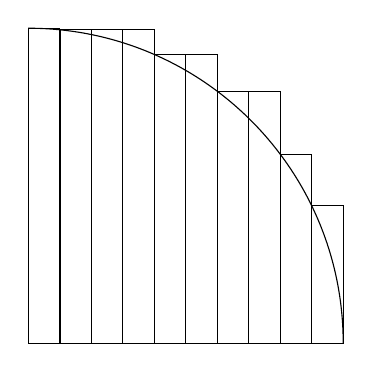
\begin{tikzpicture}
		\draw (0,0)--(0,4);
		\draw (0,0)--(4,0);
		\draw[name path=path1] (4,0) arc[start angle=0,end angle=90,radius=4cm];
		\draw[name path=path2] (0,0) rectangle(0.4,4);
		\draw[name path=path3,name intersections={of=path1 and path2}] (intersection-2) rectangle (0.8,0);
		\draw[name path=path4,name intersections={of=path3 and path1}]
		(intersection-2) rectangle (1.2,0);
		\draw[name path=path5,name intersections={of=path4 and path1}]
		(intersection-1) rectangle (1.6,0);
		\draw[name path=path6,name intersections={of=path5 and path1}]
		(intersection-1) rectangle (2,0);
		\draw[name path=path7,name intersections={of=path6 and path1}]
		(intersection-2) rectangle (2.4,0);
		\draw[name path=path8,name intersections={of=path7 and path1}]
		(intersection-2) rectangle (2.8,0);
		\draw[name path=path9,name intersections={of=path8 and path1}]
		(intersection-1) rectangle (3.2,0);
		\draw[name path=path10,name intersections={of=path9 and path1}]
		(intersection-1) rectangle (3.6,0);
		\draw[name intersections={of=path10 and path1}]
		(intersection-2) rectangle (4,0);
		\end{tikzpicture}
	\end{minipage}
	\end{figure}
\end{document}